\chapter[SCP-001 基金会]{
	SCP-001 Scantron - The Foundation \\
	SCP-001 基金会
}

\label{chap:SCP-001.the.foundation}

\begin{figure}[H]
	\centering
	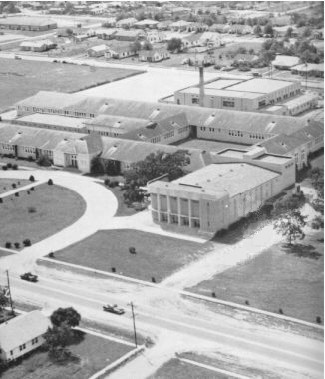
\includegraphics[width=0.5\linewidth]{images/SCP.001.the.foundation.jpg}
	\caption*{CA3的空照图,摄于最初发现后两个月。}
\end{figure}

\bb{UIU档案 0041:} 位于██████, ██的变异高中校舍(Confirmed Anomaly 3,已确认异常3号)

\bb{项目等级:}53(高侵入性、未知能力、未知性质)

\bb{特殊收容措施:}\dd{已确认异常3号(CA3)需被高于30尺的带电铁丝网所环绕,并由美国陆军第█████排守卫。任何关于CA3内部的影像资料都需尽快删除,且所有目击者都将被无限期囚禁。}

在所有情况下都不允许人员进入CA3,或与居住其中的人员沟通。但在任何时候曾经进出CA3的人都应被囚禁与审问。

由于控制项目的一个或多个实体所拥有的未知能力,对CA3的直接军事突击已经被证实是不可行的。

\bb{笔记:}\ii{这是一份摘要,不包含所有关于CA3的资讯。对CA3的详细资料请参阅UIU档案0042至0218} -██████主任

\bb{已知资讯:}特异事故处在1954年九月五日警觉到CA3的存在,当██████████高中的学生报告他们的校舍内部发生了前所未有的变化。

在发现的当下,CA3表现出数个-若非原本就存在的-异常性质:

\begin{itemize}
	\item 设施内几乎所有墙壁都被钢筋混凝土所替换,某些房间则以其他材质建造,原因不明。所有对外的窗户都从内部被掩盖。
	\item 所有课桌椅、个人财物、课本,或其他公立高中应有的物件都消失了。保险柜仍存在,但尺寸明显缩小,且是由不锈钢构成。
	\item 所有房间与设施的格局、位置与尺寸都与学校原本的蓝图不符。且房间内部经常出现看似随机的修改,被改变的房间数量仍旧不明。
	\item 发现了不少于七台的计算机,每一台都使用最先进的磁芯内存。在被分类为已确认异常之前,██████████并没有计算机。计算机内的所有资料都无法存取,且机器本身都被螺丝固定住。
	\item 礼堂被大面的钢墙阻挡而无法进入。对这个阻碍进行搬移或破坏的尝试皆以失败告终。墙壁与礼堂本身的规模与用途不明。
\end{itemize}

一支被送入CA3内部以进行完整调查的小队(CA3-O5小队)没有返回,而负责寻找前一小队的第二支队伍也是(CA3-06小队)。该设施目前被封锁,等待新的收容措施。

\bb{更新:}在最初发现的二十三天后,守卫回报CA3发出「白噪声\footnote{\bb{譯註:}White Noise,在各频率上功率都相等的“干扰”或者“噪声”}」,越接近礼堂噪声越大。五小时后,白噪声停止,但CA3内部能听见谈话声。

在深入调查之后,发现建筑内部现在包含了大量人员,所有人都看似漫无目的地在设施中游荡。值得注意的是,每个个体在外观上都与CA3-06的队员一致,但CA3内部的居民数目远超过CA3-06。囚禁或互动的试图因[机密]而失败。没有发现CA3-O5小队的十二名成员。此外,CA3的内部规划与前次调查也有明显差异。其中的运作机制尚未明了。

进一步的调查显示,大部分(或全部)产生出的物件本身都具有异常的性质。一部分的CA3-2开始看守这些物件(通称为CA3-3)或对其进行各种实验。

\bb{更新:}在前次调查的三个月后,礼堂再度发出了白噪声。这回立刻决定进行调查。发现大多数的CA3-2(对CA3内部居民的代称)聚集到礼堂的数扇门前。一个约六尺宽的圆洞出现在钢墙上,但礼堂内部仍无法观察。在0310,一个类似[机密]的物件从洞中出现,并被一名居民带走。该物件被放置在一间教室中(在先前没有观察到其开放)。这个过程持续了八小时,每三分钟出现一个新的物件。大部分进入了不同的房间或保险柜,但没有足够的人员来追踪所有物件。\footnote{
	编者 \QIS :Wiki中没有本段内容,疑为缺漏,将论坛翻译贴中的译本用于此,原帖为 \url{http://scpfoundation.123ubb.com/t1161-topic}。
}

\bb{更新:}在前次调查的两天后,三名雷同的武装「守卫」出现在CA3的入口附近。由于这些守卫能无视伤害或武器等级地制服所有派往CA3的队伍,无法进一步探索建筑。

\bb{笔记:}在守卫出现前两天搜集到的报告指出CA3-2遵循标准UIU程序来处理礼堂中出现的物件。他们对UIU标准程序的知识与CA3-O5小队一致。

\bb{更新:}在UIU追踪CA6的过程中,两名与特工Dixon(CA3-06的成员)相同的人从路边的车辆中出现并强行掳走了CA6,将他拖入车中扬长而去。往后八个小时对车辆的追踪发现他们直接驶往CA3。在抵达的时候,守卫迅速开关前门让车辆通过。CA6没有再被寻获。

\vs\hrule

\bb{UIU档案0042:}CA3发出的讯息

1965年五月15日,以下讯息以摩尔斯密码发送至标准UIU通讯频道上。敏感资料已被删改,并将每个「句子」加以编排,讯息本身并未更动。

\begin{scpbox}
你好!我们是O5议会而且我们(确保、收容、守护)我们的行动已经为你们所知而且很高兴能做朋友。以前能当你们的一份子很好但最好是有更充足的资源(更多的资源)我们会控制住收容。我们对于守卫与囚禁的行为,在此表示诚挚的歉意,我们需要保障人员与秘密:同时也对时间上的延宕道歉,无线电讯号被一或二个SCP所阻挡。预期在短时间内会有扩张,因为我们需要礼堂以外的空间(尚可但不佳)
\end{scpbox}

八小时后,收到下列讯息:

\begin{scpbox}
  扩张了!█████████联邦大楼现正运作中,需要博士守卫D人开始招募!寻找异常而且未来可能进行国际行动,研究当然可行;但跨国活动可能需要数周。此外我们O5都知道(抱歉没有O6)虽然很难探查,但媒介礼堂不是█████!再会并祝你们好运。
\end{scpbox}

更进一步的资讯参阅UIU档案0███:位于█████████, ██的变异联邦大楼(已确认异常10号)。
